\renewcommand{\chapid}{ketu}

\renewcommand{\kepler}{\project{Kepler}}
\newcommand{\plato}{\project{PLATO}}

\renewcommand{\period}{{\ensuremath{P}}}
\newcommand{\rp}{{\ensuremath{R_\mathrm{P}}}}
\renewcommand{\rate}{{\ensuremath{\Gamma}}}
\newcommand{\score}{{\ensuremath{S}}}


\chapter{%
    Searching for long-period transiting planets in the \kepler\ light curves
    using supervised classification\chaplabel{peerless}}

This \paper\ is joint work with David~W.~Hogg (NYU) and Bernhard~Sch\"olkopf
(MPIS).

\section{Chapter abstract}

Many of the most dynamically important planets have orbits longer than the
baseline of existing transit surveys (\kepler, \KT).
Future surveys (\tess, \plato) are planned to have shorter continuous coverage
that even habitable zone planets around M-dwarfs will only present a single
transit event.
Searches for these long-period transiting planets are plagued by false
signals---especially when pushed to low signal-to-noise---and statistical
studies of their population are complicated by weak constraints on the
physical parameters of the system and high rates of false positives.
We develop and present a computationally expensive but tractable method of
searching for single transits using supervised classification methods from
the machine learning literature.
For each star, we train several random forest classifiers on simulated signals
injected into different subsets of the data.
These models are evaluated on the raw photometry to assign a transit
probability at each time.
As a proof of concept, we apply this method to 3500 light curves from the
\kepler\ archival dataset and discover a previously unknown single transit
candidate.
Assuming a bound Keplerian orbit and using an informative prior on the
eccentricity, we measure a radius of $2\,R_\mathrm{J}$ and derive a weak
constraint on the orbital period.

\section{Introduction}

The transit method of exoplanet detection and characterization has been
demonstrated as a powerful method for building systematic catalogs of
exoplanets.
Despite the great success of the \kepler\ Mission with thousands of planet
discoveries \citep{Burke:2014, Rowe:2015}, current methods for exoplanet
discoveries are currently limited in the range of orbital periods that can be
studied.
Specifically, the standard transit search procedures only discover signals
with at least three observed transits \citep[for example][]{Petigura:2013,
Burke:2014, Rowe:2015}.
For \kepler, with a baseline of about four years, this sets an upper limit on
the detectable periods of just over a year.
In the Solar System, Jupiter---with a period of 12 years---dominates the
planetary dynamics and, since it would only exhibit at most one transit in the
\kepler\ data, it would be missed by most existing transit search procedures.
It is possible to discover long-period planets like this using targeted radial
velocity (RV) surveys \citep[for example][]{Butler:2006, Knutson:2014} but the
cost of implementing a systematic RV search is substantially higher than
searching the existing and forthcoming photometric data for single transits.

There are two main technical barriers to a search for single transit events.
The first is that the transit probability for long-period planets is very low;
scaling as $\propto\period^{-5/3}$ for orbital periods longer than the
baseline of contiguous observations.
Therefore, even if long-period planets are intrinsically common, they will
still be underrepresented in a transiting sample.
The second challenge is that there are substantial signals in the observed
light curves caused by stochastic processes---both instrumental
(pointing jitter, temperature variations, \etc) and astrophysical (stellar
variability, \etc)---that can masquerade as transit signals.
In practice, even using the most sophisticated systematics removal methods,
these false signal far outnumber the true single transits.

Nearly every transit search algorithm is built on the same principles and many
of the same decisions are made.
In particular, at the heart of most methods is a matched filtering step where
the likelihood of an approximate transit model is computed on a grid in the
physical parameters \citep[\kepler\ Data Processing
Handbook\footnote{\url{https://archive.stsci.edu/kepler/manuals/KSCI-19081-001_Data_Processing_Handbook.pdf}};][]{%
Petigura:2013, Huang:2013, Dressing:2015, Foreman-Mackey:2015}.
Using these methods, and substantial hand-curation, some long-period
transiting candidates have been published \citep[for example][]{Batalha:2013,
Huang:2013, Kipping:2014a}.
For more recent data releases, the community has settled on more conservative
selection criteria where candidates are required to have multiple transits
\citep[for example][]{Petigura:2013, Burke:2014, Rowe:2015}.
Even the \project{QATS} algorithm \citep{Carter:2013} for finding
quasiperiodic transits builds on much the same infrastructure.
This means that there has never been a systematic search for single transits
in the full \kepler\ dataset.

A qualitatively different approach to planet search is employed by the
\project{Planet Hunters} (PH)
project\footnote{\url{http://www.planethunters.org/}} \citep{Fischer:2012}.
PH is a ``citizen science'' project where visitors to the website look at
sections of light curve and mark the locations of transits that can be
identified visually.
Visual inspection can be a useful search technique for large single transits
because humans are able to robustly distinguish transit signals from the noise
and this project has yielded some promising long-period candidates and
confirmed planets \citep[for example][]{Wang:2013}.
One shortcoming of the PH method is that it can be difficult to fully quantify
the performance (completeness and reliability) of the search and PH does not
evaluate their users using synthetic transit signals as is now common practice
in the transit search literature.
This means that the PH sample of candidates cannot be used for robust
population inference.

We propose a transit search method that shares some similarities with the PH
model but, instead of human classifiers, we use a supervised classification
model trained on large numbers of simulated transit signals injected into
real \kepler\ light curves.
This procedure is motivated because, by definition, most randomly selected
sections of light curve contain no transits and there is an excellent physical
model for the signals of interest.
If we can train a classification model to robustly separate light curve
sections with transits from sections without then we should be able to use
this in-place of the humans to find single transit events.
This method is novel as a means to transit search and it differs substantially
from the standard methods.

Automated classification processes have been hugely successful in the machine
learning literature.
% when applied to the right datasets \dfmtodo{cite some things}.
Many astronomical problems can't be naturally solved by the standard machine
learning models because of their heterogeneous character and heteroscedastic
uncertainties.
The search for single transits, however, is an excellent use case when applied
with care.
The noise in the light curve of a given star is relatively consistent for the
full baseline of observation and we have a very good physical generative model
for the transit signal so we can simulate arbitrarily large sets of training
examples.

In the training step, a Random Forest (RF) classifier is trained to
distinguish---based only on the light curve itself---between sections of light
curve that contain transits from sections of the same size that do not.
This model is then used to find candidates in left-out sections of the light
curve.
In principle, this model can capture arbitrarily complicated non-linear
structure in the decision space and if the training set is large and complete
it will ``learn'' the shape of a physical transit.
In practice, classification algorithms like this also require a complete set
of ``negative'' training examples so further vetting using physical models
is necessary.

In \sect{est}, we extrapolate a recent model of the distribution of exoplanets
to the long periods considered in this \paper.
Using an approximate but realistic model for the detection efficiency of a
search for single transits, we estimate that $\sim 60$ single transit events
should be detectable in the archival \kepler\ dataset.
In \sect{data}, we describe the data and outline the structure exploited by
our transit search procedure.
In \sect{rfc}, we briefly describe the Random Forest classification framework
and in \sect{search} we outline the steps used to apply this model for transit
search.
This method requires the setting of many tuning parameters and the
optimization of these choices is both computationally and intellectually
challenging so in \sect{tuning} we discuss some steps in this direction.
In \sect{demo}, we demonstrate the feasibility of this method, present a
single transit discovery, and indicate some interesting weaknesses of the
method.
In \sectionname s~\sectref{params} we describe the parameter estimation that
is possible given a single transit.

% and outline the prospects for exoplanet
% population inference given a catalog of single transit discoveries.


\section{Estimated yield}\sectlabel{est}

Before the launch of the \kepler\ Mission, \citet{Yee:2008} predicted the
yield of single transit events based on the planet occurrence rates estimated
based on small catalog of radial velocity discoveries \citep{Butler:2006} and
a fit to their occurrence rate \citep{Cumming:2008}.
Using these early results and the pre-launch specifications of the \kepler\
Mission, \citet{Yee:2008} predicted that \kepler\ would discover $\sim 6$
single transit events in the full dataset.
Now that the Mission is complete and we have better estimates of the
occurrence rate and distribution of planets \citep[for example][]{Dong:2013,
Petigura:2013, Foreman-Mackey:2014, Dressing:2015}, we can update the
predicted yield for single transit events in the \kepler\ light curves.
To make this estimate, we extrapolate the distribution of large planets on
relatively short orbits out to longer periods, taking detection efficiency
and the survey and targeting properties into account.

We will base our estimate on an assumed model $Q_k(\rp,\,\period)$ for the
absolute probability of detecting a planet with radius \rp\ and period
\period\ orbiting the star $k$, and the occurrence rate distribution
\begin{eqnarray}
\rate (\rp,\,\period) &=& \frac{\dd N}{\dd\ln\rp\dd\ln\period} \quad,
\end{eqnarray}
the expected number of planets per star, per logarithmic radius, per
logarithmic period.
Given these two quantities, the expected number of single transits in the
\kepler\ data is given by
\begin{eqnarray}
N &=& \sum_{k=1}^K N_k
\end{eqnarray}
where the sum is over the $K$ stars in the sample and $N_k$ is the expected
number of observable transits around star $k$
\begin{eqnarray}\eqlabel{nk}
N_k &=& \int Q_k(\rp,\,\period) \, \rate (\rp,\,\period)
    \dd\ln\rp \dd\ln\period \quad.
\end{eqnarray}
The integral in \eq{nk} is over the full range of target parameters.

For the purposes of this discussion, we assume an approximate simple detection
efficiency model with three contributions: the geometric transit probability,
the temporal transit probability, and signal-to-noise ratio threshold of the
search technique.
Assuming circular orbits, the geometric transit probability is given by
\citep{Winn:2010}
\begin{eqnarray}\eqlabel{q-geom}
Q_k^\mathrm{(geom)}(\rp,\,\period) &=& \frac{R_k}{a} \\
&=& \left( \frac{4\,\pi^2}{G\,M_k} \right)^{1/3} \, R_k \, \period^{-2/3}
\end{eqnarray}
where $R_k$ and $M_k$ are the radius and mass of the star $k$ respectively.
The eccentricity distribution of these long-period planets will affect this
transit probability \citep{Kipping:2014} but this simple prescription should
be sufficient for a rough estimate.
For long-period orbits, the temporal transit probability will be given by
\begin{eqnarray}\eqlabel{q-time}
Q_k^\mathrm{(time)}(\rp,\,\period) &=& \frac{T_k}{\period}
\end{eqnarray}
where $T_k$ is the total time that \kepler\ spent observing the star $k$.
Finally, the detection threshold depends on the detailed sensitivity of the
search procedure but we will approximate it as a simple step function in
signal-to-noise ratio of the transit.
This contribution will be given approximately by
\begin{eqnarray}
Q_k^\mathrm{(detect)}(\rp,\,\period) &=& \left\{\begin{array}{ll}
1 & \mathrm{if}\,\left(\rp/R_k\right)^2 > f\,\sigma_k \\
0 & \mathrm{otherwise}
\end{array}\right.
\end{eqnarray}
where $\sigma_k$ is an estimate of the noise in light curve of star $k$ and
$f$ is the detection threshold for the method.

Combining the detection efficiency components, the integral from \eq{nk}
becomes
\begin{eqnarray}\eqlabel{nk-2}
N_k &=& \left( \frac{4\,\pi^2}{G\,M_k} \right)^{1/3} \, R_k \, T_k
    \int_{\rp_\mathrm{min}} ^{\rp_\mathrm{max}} \frac{\dd\rp}{\rp}
    \int_{\period_\mathrm{min}} ^{\period_\mathrm{max}}
        \period^{-8/3}\,\rate(\rp,\,\period) \dd\period
\end{eqnarray}
where all the integration limits are set by the target parameter space.
Because of the detection probability threshold, $\rp_\mathrm{min}$ can be no
smaller than $R_k\,\sqrt{f\,\sigma_k}$.
\citet{Dong:2013} used the catalog of short period transiting planets found
by \kepler\ to constrain a model for the occurrence rate of large planets of
the form
\begin{eqnarray}
\rate(\rp,\,\period) &=& C\,\left(\frac{\period}{10\,\mathrm{d}}\right)^\beta
\end{eqnarray}
in a set of radius bins.
Using this model, the integral in \eq{nk-2} becomes
\begin{eqnarray}
N_k &=& \left( \frac{4\,\pi^2}{G\,M_k} \right)^{1/3} \, R_k \, T_k \,
    \sum_{j=1}^J \frac{C_j}{(10\,\mathrm{d})^{\beta_j}}\,
    \ln \left( \frac{\rp_{\mathrm{max},j}}{\rp_{\mathrm{min},j}} \right) \,
    \left[ \frac{{\period_\mathrm{min}}^{\beta_j - 5/3}}{5/3-\beta_j} \right]
\end{eqnarray}
where the sum is over the $J$ radial bins studied by \citet{Dong:2013}.
It's important to note that the model used by \citet{Dong:2013} is given in
base-10 logarithms so the units must be converted to natural logarithms as
appropriate.

Assuming the stellar parameters provided by the NASA Exoplanet
Archive\footnote{We downloaded the \texttt{q1\_q16\_stellar} table from
\url{http://exoplanetarchive.ipac.caltech.edu/} on 2015-04-03.}
\citep{Huber:2014} and approximating the stellar noise using the 15-hour CDPP
\citep{Christiansen:2012}, \fig{predict} shows the extrapolated number of
transiting planets with $1500\,\mathrm{d} < \period < 5000\,\mathrm{d}$ based
on the \citet{Dong:2013} power-law model.
For a detection threshold $f\sim10$, the expected number of single transit
events in the \kepler\ light curves is $\sim 60$.

This results is much more optimistic than the pre-launch estimate from
\citet{Yee:2008} for a few reasons.
One effect is that, the \kepler\ Mission ran for more than four
years---longer than the fiducial Mission goal---and $\sim190,000$ stars were
targeted for nearly the full baseline instead of the original 100,000.
\dfmtodo{Explain the other reasons.}

\begin{figure}[p]
\begin{center}
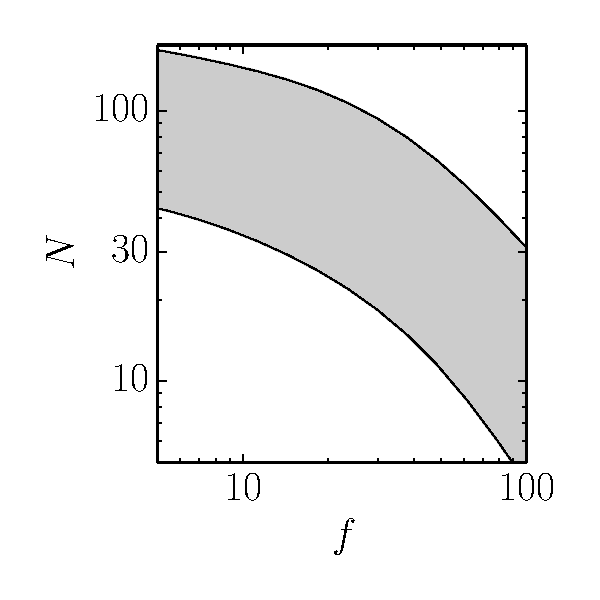
\includegraphics{figures/peerless/predict.pdf}
\end{center}
\caption[The expected number of single transit events]{%
The expected number of single transit events---extrapolated from the
\citet{Dong:2013} power-law model fit to the shorter period \kepler\
candidates---as a function of the effective signal-to-noise threshold of the
search procedure.
The shaded region indicates the uncertainties propagated from the model
parameters.
\figlabel{predict}}
\end{figure}


\section{Data preparation}\sectlabel{data}

The \kepler\ Mission measured photometric time series for about 190,000 stars
at half-hour cadence for a baseline of over four years.
We aim to search these light curves for single transits of long-period planets
and single eclipses of binary stars.
These data are made available on
MAST\footnote{\url{https://archive.stsci.edu/kepler/}} and, for each target,
we downloaded the full set of long cadence light curve files provided by Data
Release 24 \citep{Thompson:2015}.
From these files, we extracted the PDC time series and split them into
``sections'' with no more than ten contiguous missing or flagged data points.
The PDC light curves have been corrected for the instrumental effects caused
by the spacecraft using a data-driven model of the focal plane
\citep{Stumpe:2012, Smith:2012}.
Crucially, an attempt is also made by the PDC procedure to remove sharp
instrumental artifacts like ``sudden pixel sensitivity dropouts (SPSDs)''.
The success rate of this correction procedure is much higher than in earlier
data releases but, as discussed in \sect{demo}, there remain some cases that
are not properly accounted for.

The goal of this project is to discover the transits of long-period planets
that have not yet been discovered.
Therefore, when studying the light curve of an eclipsing binary star or a star
with known transiting planet candidates---on shorter periods---we also remove
all the in-transit data for the candidate using the parameters provided by the
\project{NASA Exoplanet
Archive}\footnote{\url{http://exoplanetarchive.ipac.caltech.edu/}; We
downloaded the \texttt{cumulative} table of \kepler\ Objects of Interest on
2015-03-25.}.



\section{Random forest classification}\sectlabel{rfc}

A common task in the machine learning literature is called \emph{supervised
classification} where the goal is to separate objects into classes
represented by sets of labeled examples.
In the astronomy literature, supervised classification has been used for
variable star classification \citep{Richards:2011} star--galaxy separation
\citep{Fadely:2012}, galaxy morphology prediction \citep{Dieleman:2015}, and
other applications.
In each of these problems, there are a set of measurements that have been
assigned classes---by some other method; often manually---and the goal is to
transfer these labels to a set of observations that have not yet been
labeled.
For a more in-depth discussion of the application of these techniques in
astronomy, the interested reader is directed to \citet{Ivezic:2013}.

In our problem of transit search, we want to ``label'' sections of light curve
with either the \texttt{transit} or \texttt{no transit} class.
This problem doesn't fall under the standard format of a supervised
classification problem because very few long-period transits have actually
been observed or classified.
We do think, however, that we have a good physical generative model for the
signal of interest and most of the observations of each star have no transits.
Therefore, we train the model on simulated signals.

The Random Forest (RF) classification model \citep{Breiman:2001} is a popular
model in the machine learning community where it is a common go-to model for
basic classification tasks.
It has also been applied with great success in astronomy \citep[for
example][]{Richards:2011, Richards:2012, Jenkins:2014}.
The RF model works by fitting an ensemble of decision trees to randomly
selected subsamples of the training dataset.
Each tree in the forest is ``grown'' by greedily choosing decision boundaries
that optimize the separation of the training data in randomly selected
subsets of the features until the separation is complete, each leaf contains
only one class or, at most, a fixed number of samples.
At each branch, the decision boundary is set by maximizing either the entropy
or the ``gini'' coefficient.

We use the \project{scikit-learn} \citep{Pedregosa:2011} version of the RF
classification algorithm\footnote{Specifically we use the
\texttt{RandomForestClassifier} object;
\url{http://scikit-learn.org/stable/modules/generated/sklearn.ensemble.RandomForestClassifier.html}.}
implemented in \project{Python}.
This implementation has state-of-the-art speed and
performance\footnote{\url{http://blog.explainmydata.com/2014/03/big-speedup-for-random-forest-learning.html}}
while maintaining a flexible and user-friendly interface.


\section{Search methodology}\sectlabel{search}

Now, we will apply the RF classification model to search for single transits
in \kepler\ light curves.
The basic structure of the problem, applied to the light curve of a single
star, is:
\begin{enumerate}

{\item {\bf train} a classifier on simulated signals injected into a subset of
the light curves sections,}

{\item {\bf validate} the model on signals injected into a different subset of
the data to estimate the precision of the results,}

{\item {\bf test} the classifier by applying it to a final subset of the
data---disjoint from the previous two sets---to predict the class
(\texttt{transit} or \texttt{no transit}) of each light curve section, and}

{\item iterate until the entire light curve has been classified.}

\end{enumerate}
This means that searching a single light curve involves training, validating,
and testing at least 3 RF models.
In practice, we find that it is sufficient to split the data (intelligently)
into 3 disjoint subsets so that we need only train 3 classifiers for each
star.

A key assumption of this model is that the classes are sufficiently
represented in feature space.
In other words, the training set must span both of the classes.
Given a large enough training set, this is not difficult for the
\texttt{transit} class; we can simulate a transit for any combination of
physical parameters.
This is much more difficult for the \texttt{no transit} class.
Since we don't have a generative model for the stellar and instrumental
variability or other artifacts, we cannot simulate negative examples that
cover the full space of possibilities.
Instead we are using sections of real light curves as the \texttt{no transit}
examples.
This means that there are a finite number of samples available for training
and validation, and if there is a qualitatively different signal in the test
set that is not generated by a transit, the model is at risk of unpredictably
misclassifying that section.
This problem can be largely mitigated by careful splitting of the dataset---as
described below---but there are inevitably some false signals that are not
properly accounted for.

The following \sectionname s detail the application of this search procedure
from the training set simulations through to the candidate selection.
These candidates are then vetted by hand although more robust methods should
be possible as discussed in \sect{vetting}.
Finally, \sect{features} explores alternative representations of the data or
features.


\subsection{Splitting the dataset}\sectlabel{split}

It is crucial that the model used to test for transits in a raw \kepler\
light curve not be trained on the same data.
We must split the light curve of each star into 3 disjoint sets.
For the model to work well, we require that the signals induced by
variability, noise, and other systematics be consistent between splits.
It is, therefore, necessary that we assign the splits carefully.
As discussed in \sect{data}, a light curve can be separated naturally into
``sections'' of nearly contiguous measurements; these are the base unit for
splitting the dataset.
For the typical \kepler\ target, this division is finer than month long
chunks and there are about 100 sections for each light curve.
Each light curve section is cut out of a specific ``quarter'' and each quarter
was observed during a specific ``season''.

These divisions are relevant to this discussion because the spacecraft
pointing across a quarter was extremely precise and the photometric aperture
is fixed to the same pixels for the full quarter.
Therefore, the instrumentally-induced systematics tend to be qualitatively
consistent on quarter-long time scales.
Every three months, the \kepler\ spacecraft rolled by 90~degrees causing the
stars to end up on a different detector every quarter.
This means that while the astrophysical variability should be shared between
quarters at some level, the instrumental effects can be very different.
A year later, however, the spacecraft returned to the original pointing.
As a result, the data quality is also similar for observations made in the
same season.

In order to take advantage of the natural structure of the observations, we
try to evenly distribute observations from each quarter and season across the
three sets.
When this is not possible (with Quarter 0, for example), we randomly assign
the section to a split.


\subsection{Transit simulations}

As mentioned previously, we train the RF classification models on a set
simulated transit signals injected into real light curves and a set of light
curve sections assumed to contain no transits.
For each data split, we construct a set of 20,000 \texttt{transit} samples and
an equal number of \texttt{no transit} examples.
Each of these samples is generated by randomly selecting a section of 201
contiguous flux measurements from the split.
Since we expect most of the systematic variability to be symmetric in time, we
augment the training set by reversing the time series for half of the samples.
This is analogous to image processing methods that exploit rotation and
translational symmetries \citep[for an example from astronomy
see][]{Dieleman:2015}.

To generate the \texttt{transit} examples, we simulate the transit signal
induced by the physical orbit of a large planet.
The specific distribution of simulation parameters is listed in \tab{params}.
In these simulations, we take limb darkening and integration time into
account\footnote{\url{https://github.com/dfm/transit}}
\citep{Mandel:2002, Kipping:2010}.
For the purposes of this \paper, we only simulate circular orbits under the
assumption that a single transit of a planet on an elliptical orbit would be
nearly identical to a circular orbit at a different period.

The dataset will still have some missing or flagged fluxes.
In order to account for these missing points, we linearly interpolate these
values based on their neighbors.
For consistency, we perform the interpolation on the training set \emph{after
injecting the synthetic transit signals}.
Before passing the light curve sections to the model at any stage, we
normalize the section by its empirical median and take the logarithm of the
fluxes.
This normalization appears to yield better performance in some test cases but
better performance might be achieved using optimized methods.
This choice is discussed further in \sect{params}.

\begin{table}[htbp]
\begin{center}
\begin{tabular}{lcc}
\toprule
Parameter & Units & Distribution \\
\midrule

limb darkening parameters $q_1$ and $q_2$ & --- & $q \sim U(0,\,1)$ \\
orbital period \period & days & $\ln \period \sim U(\ln 1500,\,\ln 5000)$ \\
reference transit time $\delta t$ & days & $\delta t \sim U(-0.15,\,0.15)$ \\
planet radius \rp & $R_\oplus$ & $\ln \rp \sim U(\ln 5,\,\ln 20)$ \\
impact parameter $b$ & --- & $b \sim U(0,\,1)$ \\

\bottomrule
\end{tabular}
\end{center}
\caption[Distribution of physical parameters used for simulated signals]{%
The distribution of physical parameters for the injected signals.
The limb darkening parameterization is given by \citet{Kipping:2013a}.
\tablabel{params}}
\end{table}


\subsection{Training, validation, and testing}\sectlabel{train}

For each subset of the data, we train a RF classifier on the 40,000 training
examples generated from the light curves in that split.
The \texttt{RandomForestClassifier} implementation from \project{scikit-learn}
has several tuning parameters that could be optimized using cross-validation
but we find acceptable performance in most cases using fixed values.
Specifically, we use a forest with 1000 trees by setting
\texttt{num\_estimators = 1000}.
We discuss this choice and the settings for other parameters in more detail in
\sect{params}.

Using this classifier, fit to one of the light curve subsets, we validate its
performance on each set of simulations from the two other splits.
This results in two precision--recall curves for the classifier.
The \emph{precision} is an empirical measurement of the sample purity (or
false positive rate) and \emph{recall} is a measurement of the completeness
(the probability of detecting a true signal).
Since the RF classifier scores each class and with a continuous value \score\
between 0 and 1, both precision and recall can be tuned by changing the
threshold value of \score\ above which the signal is considered a candidate.
For each model--validation set pair, we ambitiously choose the threshold in
order to obtain a precision of 100~percent.
The result of this procedure applied to the three splits is three classifiers
with two score thresholds each.

Each of these six models has been fit using two splits so we then apply it to
the raw light curves (without injected signals) from the remaining, untouched
splits.
This yields a \texttt{transit} class score as a function of transit time and
any points above the detection threshold are passed along to the candidate
selection procedure.

At this point, there are two class predictions from two different models for
every light curve section.
Any section that is classified as \texttt{transit} by \emph{both models} is
accepted as a single transit candidate.

% \dfmtodo{make a figure}


\subsection{Candidate vetting}\sectlabel{vetting}

While the search procedure described in the previous sections is quite robust
to false alarms, single transit events are extremely rare (as discussed in
\sect{est}) and because of substantial violations of the model assumptions,
false signals continue to outnumber the true signals in this catalog of
candidate transits.
To mitigate this problem, we manually inspect the light curves of candidate
signals.
As future work, we expect to automate this procedure by fitting a physical
transit model and comparing it to simple models of stellar variability and
instrumental artifacts.
For this \paper, however, the catalog of candidates is sufficiently small that
manual inspection is tractable.
As demonstrated in \sect{demo}, the most common misclassifications are caused
by astrophysical variability but some remaining systematic effects are also
incorrectly labeled as candidates.


\subsection{Feature selection}\sectlabel{features}

In many supervised classification problems, a sophisticated feature
extraction method is used to improve the performance of the procedure.
For this specific problem, we find excellent performance using the 201
normalized flux values as the features.
The depth of the transit and the noise in the light curve is not irrelevant
to detection so we don't normalize the features to unit variance in the
standard way.
Instead, we normalize each sample (feature vector) by it's empirical median
value and take the logarithm.
Another option for a feature set could be the Fourier transform or wavelet
transform of the light curve section.
Alternatively, the spectrogram of the fluxes in a larger window.
We have experimented briefly with these options but find similar performance
on the cases that we tested.


\section{Tuning parameters}\sectlabel{tuning}

Many choices need to be made in building this search procedure.
Each of these choices can be specified by a set of parameters that can be
tuned to optimize the method.
In order to tune these parameters, we must decide on a quantitative
measurement of the ``performance''.
The goal is, of course, to \emph{robustly discover transiting planets}.
In other words, the aim is a procedure that maximizes both \emph{recall} and
\emph{precision}.

As discussed previously, recall is the probability, integrated across the full
parameter space of interest that a true transit signal will be detected by the
method.
In astronomy, this quantity is generally called the completeness or detection
efficiency and it is routinely measured for transit surveys
\citep{Petigura:2013, Dressing:2015, Foreman-Mackey:2015}.
On the other hand, precision is the probability that a positive classification
will be true.
In astronomy, precision is generally hard to measure because we rarely have
access to the ground truth.
For this problem, correctly computing the recall is impossible because we
never know that \emph{there is definitely no transit} at a given time in the
light curve.

What's more, it is not in general possible to maximize both recall and
precision because transit signals are not completely separable from false
positives.
This means that, as the recall of the method improves, the false positive rate
will also increase, reducing the precision.
We must, therefore, choose a trade-off between recall and precision that
represents our objective.
The informal tradition in the transit search literature is to build a
procedure that maximizes the recall at an extremely high ($\sim 100$~percent)
fixed precision.

The main tuning parameters of the method are as follows:
\begin{itemize}

{\item \emph{the number of training and validation examples for each data
split} --- The performance of most classification models improves drastically
as the size of the training set increases but in this case we are limited by
the number of \texttt{no transit} samples that are available since we have no
generative model for the variability and systematics.
For this \paper, we choose 20,000 positive \texttt{transit} samples per split
and an equal number of negative examples.}

{\item \emph{the range of physical parameters used to simulate the transit
signals} --- The search will be most sensitive to transits with parameters
spanned by the training set but training on too many low signal-to-noise
examples in noisy light curves leads to decreased precision.
The parameter ranges used for the demonstrations here are given in
\tab{params}.}

{\item \emph{tuning parameters of the RF implementation} --- The
\texttt{RandomForestClassifier} implementation has a few tuning parameters.
The most important of these seems to be \texttt{num\_estimators}, the number
of decision trees used in the forest.
Increasing \texttt{num\_estimators} leads to substantial computational cost
with diminishing returns on the search performance.
Otherwise, there are a few parameters (for example, \texttt{max\_features},
\texttt{min\_samples\_split}, and \texttt{min\_samples\_leaf}) that can be
used to regularize the model but we have found that the performance is
insensitive to these choices.
As a trade-off between performance and computational cost, we set
\texttt{num\_estimators = 1000} in all the examples shown in this \paper.}

\end{itemize}
In detail, the optimal set of decisions and parameter settings will be
different for every target---and probably even for every permutation of the
data splits.
In practice, we find that the performance of the search is fairly insensitive
to most of these choices so we choose parameters that seem to work well in
most cases and leave optimization for future work.


\paragraph{Estimating the precision}

We estimate the precision of each RF classification model on the validation
set as described in \sect{train}.
As discussed in that \sectionname, we choose a target precision to
100~percent and set the score threshold accordingly.
This estimate is only applicable to the test set under two major assumptions.
The first is that all transiting planets with more than one transit and a
large signal-to-noise ratio have been previously discovered by one of the many
transit searches applied the \kepler\ dataset \citep{Burke:2014, Rowe:2015}.
This is a safe assumption because, for large planets, these surveys are all
largely complete out to periods yielding only 2 or 3 transits in the \kepler\
baseline \citep[for example][]{Petigura:2013}.
The second assumption is not always valid so it makes this estimate of the
precision only approximate and not completely reliable.
This assumption is that the noise processes in the data are stationary.
In other words, the transit-like noise signals in the training and validation
sets must be ``similar'' to the signals in the test section.
This constraint is nearly satisfied when the PDC light curves are used
(\sect{data}) and the data are split carefully (\sect{split}).
As demonstrated by the mis-classifications shown in \sect{demo}, however, it
is clear that violations to this rule do exist in the data and final vetting
of the candidates must be applied using a physical understanding of the
signals.


\section{Preliminary results}\sectlabel{demo}

As a demonstration of the feasibility of this method to search for single
transit events, we selected 3500 bright, Sun-like stars based on the revised
stellar parameters collected and measured for a recent \kepler\ data release
\citep{Huber:2014}.
The targets were selected in the parameter range
\begin{itemize}

\item effective temperature:
        $4100\,\mathrm{K} < T_\mathrm{eff} < 6100\,\mathrm{K}$,

\item surface gravity:  $4.0 < \log g < 4.9$, and

\item \kepler\ magnitude: $15 > K_\mathrm{p} > 10$.

\end{itemize}

This search results in 596 candidate transits in the light curves of these
3500 stars.
The vast majority of these candidates are misclassified false positives and
many of them are caused by astrophysical sources.
To weed out known astrophysical sources, we cross-match this list against
known eclipsing binary stars \citep{Matijevic:2012} and stars with substantial
variability \citep{McQuillan:2014}.
Removing these signals results in 273 candidates.
Of these candidates only one (KIC 10602068) is a convincing transit and the
others all appear to be caused by systematic effects, instrumental or
astrophysical.
\Fig{candidates} shows some representative candidate signals from this final
list.

\paragraph{Failures}

\dfmtodo{Add some discussion of the failures and make suggestions for better
vetting techniques.}


\begin{figure}[p]
\begin{center}
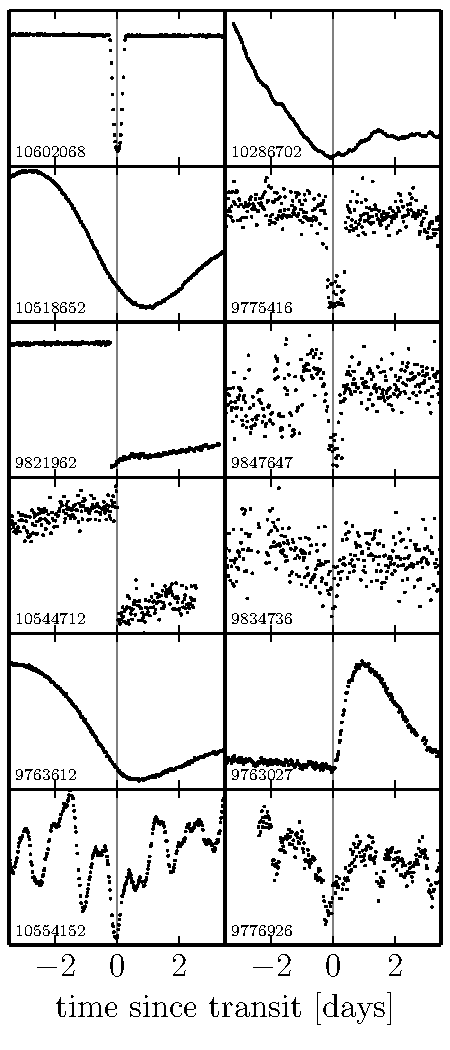
\includegraphics[width=0.5\textwidth]{figures/peerless/candidates.pdf}
\end{center}
\caption[Light curves of reprensentative single transit candidates]{%
Some representative light curve sections that were labeled as candidates by
the single transit search.
The light curve in the top-left panel is a convincing transit signal but the
other panels all appear to be caused by stellar variability or instrumental
effects.
\figlabel{candidates}}
\end{figure}



\section{KIC 10602068: A discovery}\sectlabel{params}

In the 3500 light curves we searched for this \paper, we discovered one
convincing single transit signal at $830.8093\pm0.0002$~KBJD in the light
curve of the 14.9~Kep-mag G-dwarf KIC 10602068.
Despite the fact that this is a very large signal, its discovery has never
been reported.
Given the estimate of $\sim 60$ detectable single transits in the full
\kepler\ archival dataset, we do expect about one discovery in 3500 light
curves.

Even though only one transit is observed, if we assume that the transit is
caused by a body on a Keplerian orbit around the host star, we can place
constraints on the physical properties---even the orbital period---of the
transiting candidate.
This technique is similar in spirit to the ``photoeccentric effect''
\citep{Dawson:2012} and ``asterodensity profiling'' \citep{Kipping:2012}.
The fundamental principle is that the transit duration is a measurement of
the instantaneous velocity of the planetary motion and this yields a
constraint on the orbital period when combining this with a measurement of the
stellar density and a prior on the eccentricity of the orbit.

The photometrically derived physical properties for this star place it as a
G-dwarf with a mass and radius of about 90~percent Solar \citep{Huber:2014}.
Using these constraints and a beta function prior on the eccentricity of the
orbit \citep{Kipping:2013}, we run Markov Chain Monte Carlo
\citep{Foreman-Mackey:2013} to sample the posterior probability for the
physical parameters of the system.
In this analysis, we take limb darkening and the finite exposure time into
account \citep{Mandel:2002, Kipping:2010, Kipping:2013a}.
The results of this chain marginalized into the relevant physical dimensions
are shown in \fig{corner}.
The radius of the transiting body is measured to be $2.1 \pm
0.4\,R_\mathrm{J}$.
The period is very weakly constrained above a lower limit of
$760\,\mathrm{days}$---set by the fact that a second transit is not
detected---with 68~percent of the posterior mass in the range $760\,\mathrm{d}
< \period < 1347\,\mathrm{d}$.

Given the large radius of this candidate, it is probably stellar in nature
instead of planetary but this could be easily confirmed using radial velocity
follow-up.

\begin{figure}[p]
\begin{center}
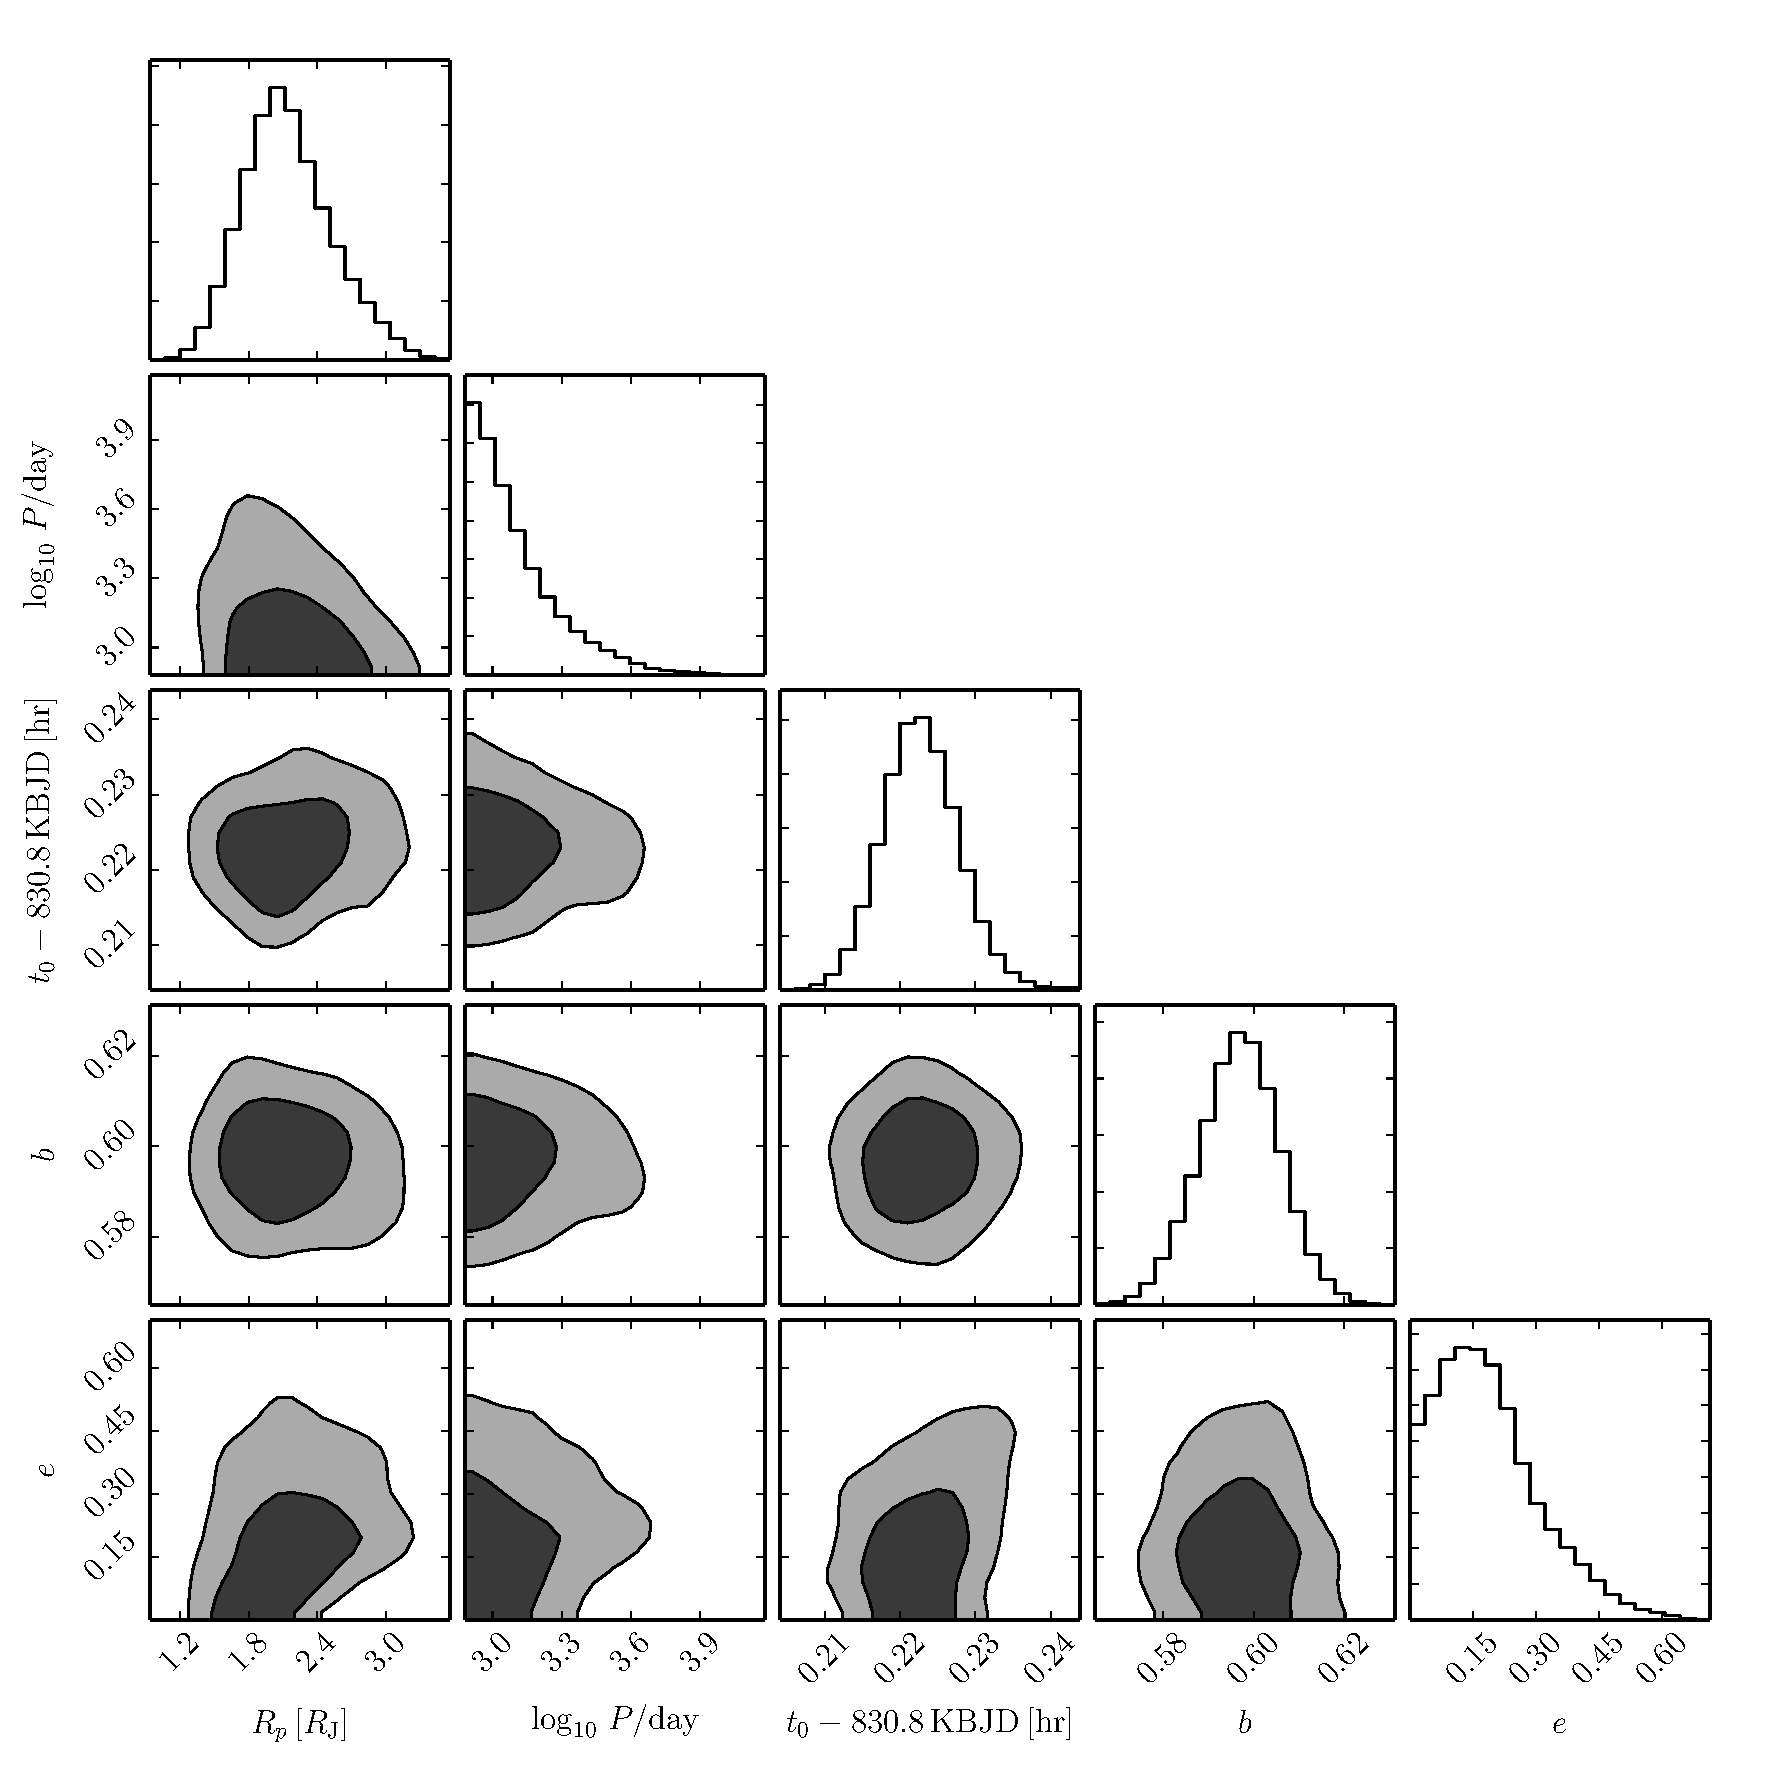
\includegraphics[width=\textwidth]{figures/peerless/corner.pdf}
\end{center}
\caption[Posterior constraints on the physical parameters of the transiting
companion of KIC 10602068]{%
Posterior constraints on the physical parameters of the body transiting KIC
10602068 assuming a bound Keplerian orbit.
\figlabel{corner}}
\end{figure}


% \section{Prospects for population inference}\sectlabel{exopop}

% Based on our single transit discoveries, we now want to place a limit on
% the occurrence rate of long-period planets.
% Since we only have one discovery thus far, we'll make the simplifying
% assumption that the rate is flat in log-period and log-radius in the range
% $1000\,\mathrm{d} < \period < 5000\,\mathrm{d}$ and $5\,R_\odot <
% 20\,R_\odot$.
% For this distribution, \citet{Foreman-Mackey:2014} derived the analytic
% maximum likelihood result
% \begin{eqnarray}
% \rate &=& \frac{N_\mathrm{obs}}{\int Q(w)\dd w}
% \end{eqnarray}
% where $\rate$ is the occurrence rate per natural logarithm in period and
% radius, $N_\mathrm{obs}$ is the number of detections, and the integral is over
% the completeness measurements for every star that has been searched.
% If we make the simplifying assumption that the detectability of a transit
% depends on period only through Equations~(\eqref{q-geom})
% and~(\eqref{q-time}), then this integral becomes
% \begin{eqnarray}
% \int Q(w)\dd w &=& \sum_{k=1}^K
%     \left( \frac{4\,\pi^2}{G\,M_k} \right)^{1/3} \, R_k \, T_k \, Q_k \,
%     \int \period^{-8/3}\,\rp^{-1} \dd\rp\dd\period \\
%  &=& \sum_{k=1}^K
%     \left( \frac{4\,\pi^2}{G\,M_k} \right)^{1/3} \, R_k \, T_k \, Q_k \,
%     \ln \left(\frac{\rp_\mathrm{max}}{\rp_\mathrm{min}}\right)
%     \frac{3}{5} \,
%     \left[{\period_\mathrm{min}}^{-5/3} - {\period_\mathrm{max}}^{-5/3}\right]
% \end{eqnarray}
% where the sum is over all the targeted stars.


\section{Discussion}\sectlabel{discussion}

The discovery and characterization of transiting planets based on a single
transit event is crucial for the future of transiting exoplanet surveys.
Many of the most dynamically influential planets---like Jupiter in our Solar
system---exhibit only a single transit in the full observational baseline of
the \kepler.
This will become even more of a problem as upcoming surveys move to shorter
contiguous observations.
For example, the \tess\ Mission is planned to get full-sky coverage at
half-hour cadence but most of the sky will only be targeted for a month.
This means that even habitable zone planets orbiting cool stars will transit
their host \emph{at most once in the entire lifetime of the Mission}!

To date, no methods exist for systematically and robustly discovering single
transit events based on large photometric surveys.
In this \paper, we present a novel and conceptually unique solution to this
problem drawing on machine learning methods for supervised classification.
This method has immense potential because it can be designed to be very robust
to false positives and it can exploit the detailed shape of physical transits.

Despite the fact that single transits are unlikely even if these long-period
planets are intrinsically common, we estimate that $\sim 60$ events should be
detectable in the \kepler\ archival dataset by extrapolating recent models of
planet occurrence rates and taking selection effects into account.
When applied to 3500 light curves from the \kepler\ dataset, this method
recovers one previously unknown single transit event at
$830.8093\pm0.0002$~KBJD in the light curve of KIC 10602068.
This rate is consistent with the predicted yield of 60 events in the full
dataset of 190,000 light curves.

Assuming a bound Keplerian orbit, we place constraints on the physical
properties of this transit candidate KIC 10602068.01.
Using photometrically derived stellar properties, we find that this candidate
has a radius of $2.1 \pm 0.4\,R_\mathrm{J}$ placing it as a very large planet
or brown dwarf or a small star.

This method for transit search is built using supervised classification and
its performance relies on several strong assumptions about the datasets and
these assumptions are sometimes violated leading to some transit-like signals
that appear to be caused by noise to be misclassified as transits.
The most severe assumption is that the noise properties of the data are
stationary.
In other words, we assume that variability in one subset of a light curve is
completely spanned by the variability in the other sections.
This assumption is, in general, false because the stochastic processes that
cause stellar variability are complicated and non-stationary and the detector
is plagued by non-negligible catastrophic changes in sensitivity and response.
We attempt to mitigate this problem by using light curves that have been
preprocessed to remove most of the instrumental effects and carefully dividing
the data into subsets but some false positives are still incorrectly
identified as candidates.

One possible method for reducing the false positive rate would be to augment
the training dataset using heuristic simulations of common false positives or
the light curves of ``similar'' stars.
Another option is to recognize that this search drastically reduces the
parameter space requiring evaluation and comparing the predictive power of
a transit model to other heuristic models including stellar variability or
instrumental effects.

As discussed in \sect{params}, many decisions were made in the application of
this method and the related hyperparameters were set heuristically.
Instead, substantial gains could be made by optimizing these choices
objectively, especially on the edge cases and methodological failures.
In particular, some different combinations of feature selection and
regularization should improve the performance.
